%%%%%%%%%%%%%%%%%%%%%%%%%%%%%%%%%%%%%%%%%%%%%%%%%%%%%%%%%%%%%%%%%%%%%%
%%  Copyright by Wenliang Du.                                       %%
%%  This work is licensed under the Creative Commons                %%
%%  Attribution-NonCommercial-ShareAlike 4.0 International License. %%
%%  To view a copy of this license, visit                           %%
%%  http://creativecommons.org/licenses/by-nc-sa/4.0/.              %%
%%%%%%%%%%%%%%%%%%%%%%%%%%%%%%%%%%%%%%%%%%%%%%%%%%%%%%%%%%%%%%%%%%%%%%

\newcommand{\commonfolder}{../../common-files}

\documentclass[11pt]{article}

\usepackage[most]{tcolorbox}
\usepackage{times}
\usepackage{epsf}
\usepackage{epsfig}
\usepackage{amsmath, alltt, amssymb, xspace}
\usepackage{wrapfig}
\usepackage{fancyhdr}
\usepackage{url}
\usepackage{verbatim}
\usepackage{fancyvrb}
\usepackage{adjustbox}
\usepackage{listings}
\usepackage{color}
\usepackage{subfigure}
\usepackage{cite}
\usepackage{sidecap}
\usepackage{pifont}
\usepackage{mdframed}
\usepackage{textcomp}
\usepackage{enumitem}


% Horizontal alignment
\topmargin      -0.50in  % distance to headers
\oddsidemargin  0.0in
\evensidemargin 0.0in
\textwidth      6.5in
\textheight     8.9in 

\newcommand{\todo}[1]{
\vspace{0.1in}
\fbox{\parbox{6in}{TODO: #1}}
\vspace{0.1in}
}


\newcommand{\unix}{{\tt Unix}\xspace}
\newcommand{\linux}{{\tt Linux}\xspace}
\newcommand{\minix}{{\tt Minix}\xspace}
\newcommand{\ubuntu}{{\tt Ubuntu}\xspace}
\newcommand{\setuid}{{\tt Set-UID}\xspace}
\newcommand{\openssl} {\texttt{openssl}}


\pagestyle{fancy}
\lhead{\bfseries SEED Labs}
\chead{}
\rhead{\small \thepage}
\lfoot{}
\cfoot{}
\rfoot{}


\definecolor{dkgreen}{rgb}{0,0.6,0}
\definecolor{gray}{rgb}{0.5,0.5,0.5}
\definecolor{mauve}{rgb}{0.58,0,0.82}
\definecolor{lightgray}{gray}{0.90}


\lstset{%
  frame=none,
  language=,
  backgroundcolor=\color{lightgray},
  aboveskip=3mm,
  belowskip=3mm,
  showstringspaces=false,
%  columns=flexible,
  basicstyle={\small\ttfamily},
  numbers=none,
  numberstyle=\tiny\color{gray},
  keywordstyle=\color{blue},
  commentstyle=\color{dkgreen},
  stringstyle=\color{mauve},
  breaklines=true,
  breakatwhitespace=true,
  tabsize=3,
  columns=fullflexible,
  keepspaces=true,
  escapeinside={(*@}{@*)}
}

\newcommand{\newnote}[1]{
\vspace{0.1in}
\noindent
\fbox{\parbox{1.0\textwidth}{\textbf{Note:} #1}}
%\vspace{0.1in}
}


%% Submission
\newcommand{\seedsubmission}{You need to submit a detailed lab report, with screenshots,
to describe what you have done and what you have observed.
You also need to provide explanation
to the observations that are interesting or surprising.
Please also list the important code snippets followed by
explanation. Simply attaching code without any explanation will not
receive credits.}

%% Book
\newcommand{\seedbook}{\textit{Computer \& Internet Security: A Hands-on Approach}, 2nd
Edition, by Wenliang Du. See details at \url{https://www.handsonsecurity.net}.}

%% Videos
\newcommand{\seedisvideo}{\textit{Internet Security: A Hands-on Approach},
by Wenliang Du. See details at \url{https://www.handsonsecurity.net/video.html}.}

\newcommand{\seedcsvideo}{\textit{Computer Security: A Hands-on Approach},
by Wenliang Du. See details at \url{https://www.handsonsecurity.net/video.html}.}

%% Lab Environment
\newcommand{\seedenvironment}{This lab has been tested on our pre-built
Ubuntu 16.04 VM, which can be downloaded from the SEED website. }

\newcommand{\seedenvironmentA}{This lab has been tested on our pre-built
Ubuntu 16.04 VM, which can be downloaded from the SEED website. }

\newcommand{\seedenvironmentB}{This lab has been tested on our pre-built
Ubuntu 20.04 VM, which can be downloaded from the SEED website. }

\newcommand{\seedenvironmentAB}{This lab has been tested on our pre-built
Ubuntu 16.04 and 20.04 VMs, which can be downloaded from the SEED website. }

\newcommand{\nodependency}{Since we use containers to set up the lab environment, 
this lab does not depend too much on our SEED VM. You can do this lab
using other VMs or physical machines. }







\newcommand{\seedlabcopyright}[1]{
\vspace{0.1in}
\fbox{\parbox{6in}{\small Copyright \copyright\ {#1}\ \ by Wenliang Du.\\
      This work is licensed under a Creative Commons
      Attribution-NonCommercial-ShareAlike 4.0 International License.
      If you remix, transform, or build upon the material, 
      this copyright notice must be left intact, or reproduced in a way that is reasonable to
      the medium in which the work is being re-published.}}
\vspace{0.1in}
}






\usepackage{longtable}
\usepackage{enumitem}
\usepackage{stackengine}
\newcommand\xrowht[2][0]{\addstackgap[.5\dimexpr#2\relax]{\vphantom{#1}}}



\newcommand{\miniVPN}{{\tt MiniVPN}\xspace}
\newcommand{\hostu}{{\tt U}\xspace}
\newcommand{\hostv}{{\tt V}\xspace}


\newcommand{\vpnFigs}{./Figs}

\lhead{\bfseries SEED Labs -- VPN Lab}


\begin{document}

\begin{center}
{\LARGE Virtual Private Network (VPN) Lab}
\end{center}

\seedlabcopyright{2006 - 2016}



% *******************************************
% SECTION
% ******************************************* 
\section{Overview}

A Virtual Private Network (VPN) is used for creating a private scope 
of computer communications or providing a secure extension of a private 
network into an insecure network such as the Internet. VPN is a widely
used security technology. VPN can be built upon IPSec or 
TLS/SSL (Transport Layer Security/Secure Socket Layer). 
These are two fundamentally different 
approaches for building VPNs. In this lab, we focus 
on the TLS/SSL-based VPNs. This type of VPNs is often referred to 
as TLS/SSL VPNs.

The learning objective of this lab is for students to master the 
network and security technologies underlying VPNs. To achieve this goal,  
students will be asked to implement a simple TLS/SSL VPN. 
Although this VPN is simple, it does include all the essential
elements of a VPN. The design and implementation of TLS/SSL VPNs exemplify
a number of security principles, including the following:

\begin{itemize}[noitemsep]
\item Virtual Private Network
\item TUN/TAP, and IP tunneling 
\item Routing
\item Public-key cryptography, PKI, and X.509 certificate
\item TLS/SSL programming
\item Authentication
\end{itemize}


\paragraph{Readings and videos.}
Detailed coverage of VPN, PKI, and TLS can be found in the following:

\begin{itemize}
\item Chapters 19, 24, and 25 of the SEED Book, \seedbook
\item Section 8 of the SEED Lecture, \seedisvideo
\end{itemize}


\paragraph{Related labs.}
We have a separate SEED lab on PKI, and another one on TLS. 
It is recommended that students finish these
two crypto labs before working on this comprehensive VPN lab. If 
students are only interested in the tunneling part of the VPN (without
the crypto part), they should use the VPN Tunneling Lab, instead 
of this one.


\paragraph{Lab Environment.} 
\seedenvironmentB
We need to use the \openssl package in this lab. The package includes
the header files, libraries, and commands. The package was 
already installed in our pre-built VM image. 





\newpage
% *******************************************
% SECTION
% ******************************************* 
\section{Lab Tasks}

In this lab, students need to implement a simple VPN for \linux. We will
call it {\tt miniVPN}. 




% -------------------------------------------
% SUBSECTION
% ------------------------------------------- 
\subsection{Task 1: VM Setup}

We will create a VPN tunnel between a 
computer (client) and a gateway, allowing the computer to securely access 
a private network via the gateway. 
We need at least three VMs: VPN client (also serving as Host U), VPN server (the gateway),
and a host in the private network (Host V). 
The network setup is depicted in Figure~\ref{vpn:fig:host2gateway}.


\begin{figure}[htb]
\begin{center}
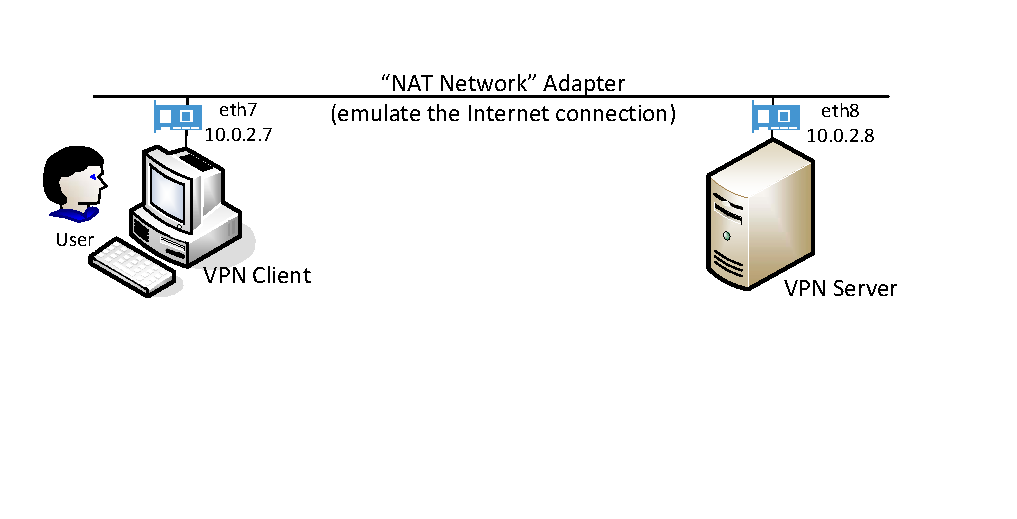
\includegraphics[width=0.9\textwidth]{\vpnFigs/Host2Gateway.pdf}
\end{center}
\caption{VM setup for this lab}
\label{vpn:fig:host2gateway}
\end{figure}
 


In practice, the VPN client and VPN server are connected via the Internet.
For the sake of simplicity, we directly connect these two
machines to the same LAN in this lab, i.e., this LAN simulates the Internet. 
We will use the ``NAT Network'' adaptor for this LAN.
The third machine, Host V, is a computer inside the private network. Users
on Host U (outside of the private network) want to communicate with Host V
via the VPN tunnel. To simulate this setup, we connect Host V to VPN Server
(also serving as a gateway) via an ``Internal Network''.  In such a setup, 
Host V is not directly accessible from the Internet; nor is it directly accessible 
from Host U. 

Note if a VM uses the ``Internal Network'' mode, VirtualBox provides no DHCP to it, so the
VM must be statically configured. To do this, click the network icon on the top-right corner
of the desktop, and select \texttt{"Edit Connections"}. You will see a list 
of \texttt{"Wired connections"}, one for each of the network adaptors used by the VM. 
For Host V, there is only one connection, but for VPN Server, we will see two. To make sure 
that you pick the one that is corresponding to the ``Internal Network'' adapter, 
You can check the MAC address displayed in the pop-up window after you have 
picked a connection to edit. 
Compare this MAC address with the one that you get from \texttt{ifconfig},
and you will know whether you picked the right connection. 

After you have selected the right connection to edit, 
pick the \texttt{"ipv4 Settings"} tab and select the 
\texttt{"Manual"} method, instead of the default \texttt{"Automatic (DHCP)"}. Click 
the \texttt{"Add"} button to set up the new IP address for the VM. See
Figure~\ref{vpn:fig:internalnetwork} for details. 



\begin{figure}[htb]
\begin{center}
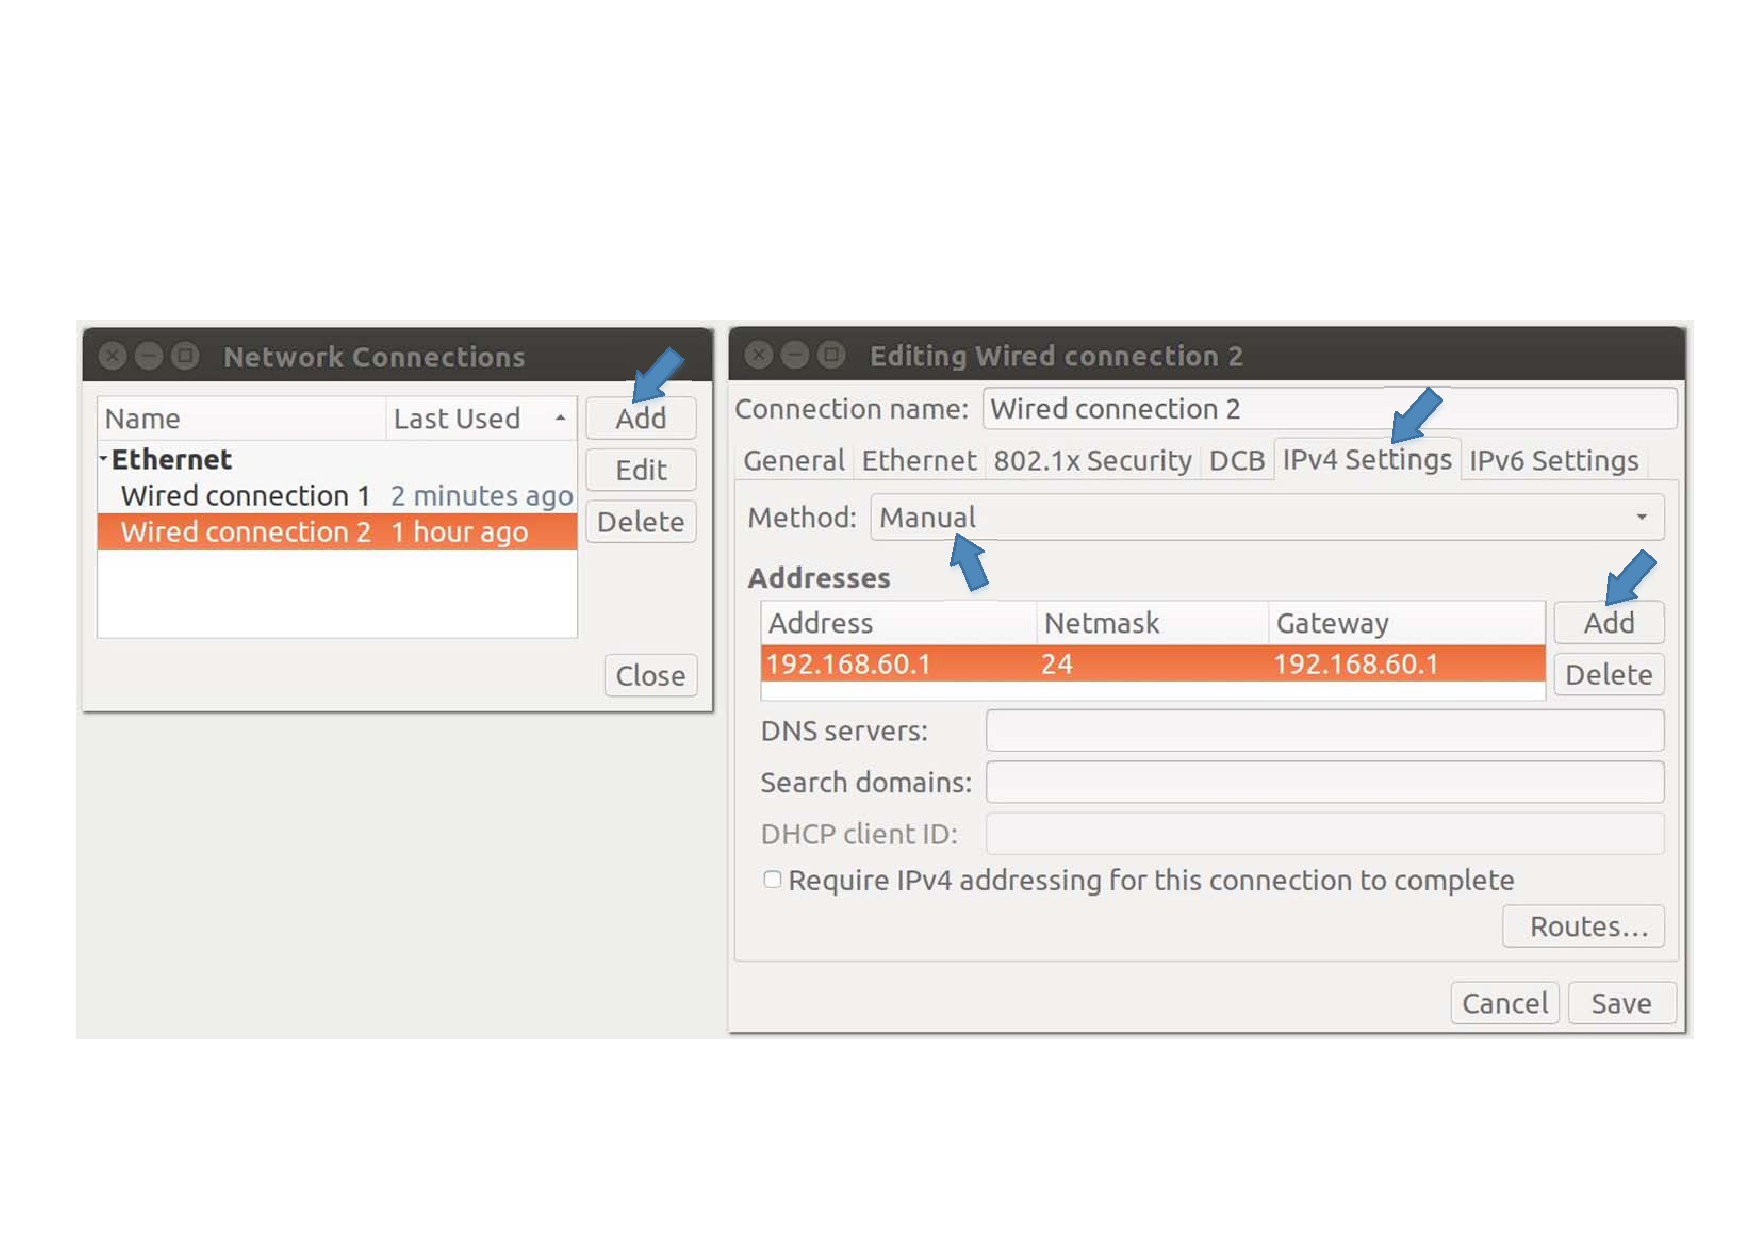
\includegraphics[width=0.8\textwidth]{\vpnFigs/InternalNetwork.pdf}
\end{center}
\caption{Manually set up the IP address for the \texttt{"Internal Network"} adaptor on VPN
Server.}
\label{vpn:fig:internalnetwork}
\end{figure}
 


% -------------------------------------------
% SUBSECTION
% ------------------------------------------- 
\subsection{Task 2: Creating a VPN Tunnel using TUN/TAP}



The enabling technology for the TLS/SSL VPNs is 
TUN/TAP, which is now widely implemented in modern operating systems.
TUN and TAP are virtual network kernel drivers; they 
implement network device that are supported entirely in software.
TAP (as in network tap) simulates an Ethernet device and it operates with 
layer-2 packets such as Ethernet frames; TUN (as in network TUNnel) simulates a
network layer device and it operates with layer-3 packets such as IP packets.
With TUN/TAP, we can create virtual network interfaces. 


A user-space program is usually attached to the TUN/TAP virtual network interface.
Packets sent by an operating system via a TUN/TAP network interface 
are delivered to the user-space program. On the other hand,
packets sent by the program
via a TUN/TAP network interface are injected into the operating system
network stack; to the operating system,
it appears that the packets come from an external source
through the virtual network interface.


When a program is attached to a TUN/TAP interface, the IP packets that 
the computer sends to this interface will be piped into the 
program; on the other hand, the IP packets that the program sends to the 
interface will be piped into the computer, as if they came from 
the outside through this virtual network interface. The program can use 
the standard {\tt read()} and {\tt write()} system calls to receive packets 
from or send packets to the virtual interface.


We have created a sample VPN client program (\texttt{vpnclient})  and 
a server program (\texttt{vpnserver}), both of which can be downloaded from
this lab's web site. 
The programs are explained in details in Chapter 16 of the SEED book titled
\textit{Computer \& Internet Security: A Hands-on Approach, 2nd Edition}; the chapter also
explains how TUN/TAP works and how to use it to create VPN.



\begin{figure}[htb]
\begin{center}
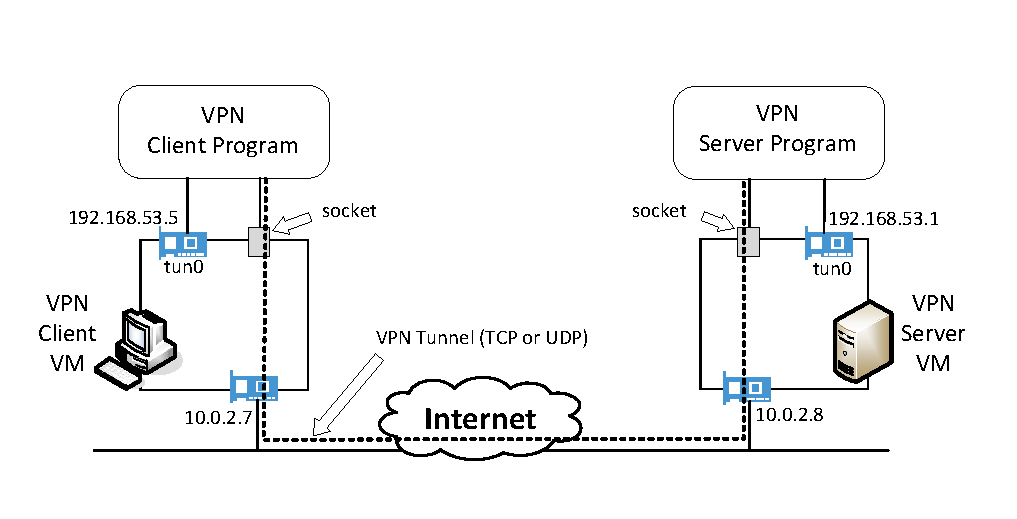
\includegraphics[width=0.9\textwidth]{\vpnFigs/ClientServerTunnel.pdf}
\end{center}
\caption{VPN client and server}
\label{vpn:fig:client_server}
\end{figure}

The \texttt{vpnclient} and \texttt{vpnserver} programs are the two ends of
a VPN tunnel. They communicate with each other using either TCP or UDP via the sockets
depicted in Figure~\ref{vpn:fig:client_server}. In our sample code, we choose 
to use UDP for the sake of simplicity.  The dotted line between the
client and server depicts the path for the VPN tunnel. 
The VPN client and server programs connect to the hosting system via a
TUN interface, through which they do two things: (1) get IP packets from
the hosting system, so the packets can be sent through the tunnel, (2) get IP packets from the
tunnel, and then forward it to the hosting system, which will forward the
packet to its final destination. 
The following procedure describes how to create a VPN tunnel 
using the \texttt{vpnclient} and \texttt{vpnserver} programs. 


\paragraph{Step 1: Run VPN Server.} 
We first run the VPN server program \texttt{vpnserver} on the Server VM.
After the program runs, a virtual TUN network interface will appear 
in the system (we can see it using the \texttt{"ifconfig -a"} command; the name of the
interface will be \texttt{tun0} in most cases, but they can be
\texttt{tunX}, where \texttt{X} is a number).   
This new interface is not yet configured, so we need to configure it by giving it an IP
address. We use \texttt{192.168.53.1} for this interface.  


Run the following commands. The first command will start the server
program, and the second command assigns an IP address to the \texttt{tun0}
interface and then activates it. It should be noted that the first 
command will block and wait for connections, 
so we need to find another window run the second command.


\begin{lstlisting}
$ sudo ./vpnserver

Run the following command in another window:
$ sudo ifconfig tun0 192.168.53.1/24 up
\end{lstlisting}

Unless specifically configured, a computer will only act as a host, 
not as a gateway. The VPN Server needs to forward packets between the private network and the 
tunnel, so it needs to function as a gateway. We need to  
enable the IP forwarding for a computer to behave like a gateway. 
IP forwarding can be enabled
using the following command:

\begin{lstlisting}
$ sudo sysctl net.ipv4.ip_forward=1
\end{lstlisting}



\paragraph{Step 2: Run VPN Client.} We now run the VPN client program on the Client
VM.  We run the following commands on this machine. The first command
will connect to the VPN server program (the server's IP address is hardcoded
inside the program, and you need to change it accordingly).
This command will block as well, so we need to find another window to 
configure the \texttt{tun0} interface created by the VPN client program.  
We assign IP address \texttt{192.168.53.5} to the \texttt{tun0} interface.   


\begin{lstlisting}
On VPN Client VM:
$ sudo ./vpnclient 

Run the following command in a different window
$ sudo ifconfig tun0 192.168.53.5/24 up
\end{lstlisting}



\paragraph{Step 3: Set Up Routing on Client and Server VMs:} 
After the above two steps, the tunnel will be established. 
Before we can use the tunnel, we need to set up routing 
paths on both client and server machines to direct the intended traffic through
the tunnel. On the client machine, we need to direct all the packets going
to the private network ({\tt 192.168.60.0/24}) towards the \texttt{tun0}
interface, from where the packets can be forwarded through the VPN tunnel.
Without this setup, we will not be able to access the private network at
all. We can use the \texttt{route} command to add an routing entry. The
following example shows how to route the \texttt{10.20.30.0/24}-bound
packets to the interface \texttt{eth0}. 

\begin{lstlisting}
$ sudo route add -net 10.20.30.0/24 eth0
\end{lstlisting}


On both client and server machines, we also need to 
set up a routing entry so all the traffic going to the \texttt{192.168.53.0/24}
network are directed to the \texttt{tun0} interface. This entry will usually be 
automatically added when we assign \texttt{192.169.53.X} to
the \texttt{tun0} interface.  If for some reasons it is not added, 
we can use the \texttt{route}  command to add it.




\paragraph{Step 4: Set Up Routing on Host V.} 
When Host V replies to a packet sent from Host U, it needs to route the
packets to the VPN Server VM, from where, it can be fed into
the VPN tunnel toward the other end. You need to find out what entry to
add, and then use  the \texttt{route} command to add the routing entry. 
Hint: when Host V receives a packet from Host U (via the tunnel), you need to know what the
source IP is in the packet; in the reply packet, the source IP becomes the
destination IP, which will be used by the routing table. Therefore, you
need to figure out the source IP of the packets from U to V. It is your
task to figure this out and set the routing correctly in this step.


\paragraph{Step 5: Test the VPN Tunnel:} After everything is set up, we can 
access Host V from Host U via the tunnel. 
Please conduct the following tests using \texttt{ping} and \texttt{telnet}; 
please  report your results. You should use Wireshark to 
capture the network traffics on all the interfaces on the client VM, 
and pinpoint which packets are part of the tunnel traffic, and
which packets are not the tunnel traffic. 

\begin{lstlisting}
On Host U:
$ ping 192.168.60.101
$ telnet 192.168.60.101
\end{lstlisting}


\paragraph{Step 6: Tunnel-Breaking Test.} 
On Host U, \texttt{telnet} to \texttt{Host V}. While keeping the
\texttt{telnet} connection alive, we break the VPN tunnel. We then type something
in the \texttt{telnet} window, and report what you observe. 
We then reconnect the VPN tunnel. What is going to happen to the
\texttt{telnet} connection? Will it be broken or resumed?
Please describe and explain your observations. 



% -------------------------------------------
% SUBSECTION
% ------------------------------------------- 
\subsection{Task 3: Encrypting the Tunnel}


At this point, we have created an IP tunnel, but our tunnel is not protected. 
Only after we have secured this tunnel, can we call it a VPN tunnel. 
This is what we are going to achieve in this task. 
To secure this tunnel, we need to achieve two 
goals, confidentiality and integrity. 
The confidentiality is achieved using encryption, i.e.,
the contents that go through the tunnel is encrypted. 
The integrity goal ensures that nobody can tamper with 
the traffic in the tunnel or launch a replay attack. 
Integrity can be achieved using 
Message Authentication Code (MAC). 
Both goals can be achieved using Transport Layer Protocol (TLS). 


TLS is typically built on top of TCP. The sample VPN client and server 
programs in Task 2 use UDP, so we first need to 
replace the UDP channel in the sample code with a TCP channel, and then establish a
TLS session between the two ends of the tunnel.  A sample TLS client
and server program (\texttt{tlsclient} and \texttt{tlsserver})   
is provided in a zip file that can be downloaded from the website. 
Instructions on how to compile and run the code
is provided in the README file included in the zip file. 
For detailed explanation of the sample
code, please read Chapter 25 of the SEED book (\textit{Computer \& Internet Security: A
Hands-on Approach, 2nd Edition}). In your demonstration, you need to use Wireshark to
capture the traffic inside the VPN tunnel, and show that the traffic is
indeed encrypted. 



% -------------------------------------------
% SUBSECTION
% ------------------------------------------- 
\subsection{Task 4: Authenticating the VPN Server}


Before a VPN is established, the VPN client must authenticate
the VPN server, making sure that the server is not a fraudulent 
one. On the other hand, the VPN server must authenticate the
client (i.e. user), making sure that the user has 
the permission to access the private network. 
In this task, we implement the server authentication; 
the client authentication is in the next task. 

A typical way to authenticate servers is to use public-key
certificates. The VPN server needs to first get a public-key 
certificate from a Certificate Authority (CA).
When a client makes a connection to the VPN 
server, the server will use the certificate to prove it 
is the intended server.  
The HTTPS protocol uses this approach to 
authenticate web servers, ensuring that you are talking to 
an intended web server, not a fake one. 


In this lab, \miniVPN should use such a method to authenticate the
VPN server. We can implement an authentication protocol (such
as TLS/SSL) from the scratch, but fortunately, \texttt{openssl} has 
taken care most of the work for us. We just need to configure 
our TLS session properly, so \texttt{openssl} can conduct the authentication
automatically for us.  

There are three important steps in server authentication: (1) verifying that
the server certificate is valid, (2) verifying that the server 
is the owner of the certificate, and (3) verifying that the server is
the intended server (for example, if the user intends to visit 
\texttt{example.com}, we need to ensure that the server is indeed 
\texttt{example.com}, not another site). Please point out what lines of the
code in your program carry out the above verifications. 
In your demonstration, you need to demonstrate two different cases regarding the 
third verification: a successful server authentication where the 
server is the intended server, and a failed server authentication where 
the server is not the intended server. 


\paragraph{Note:} Our \miniVPN program should be able to communicate with
VPN servers on different machines, so you cannot hardcode the hostname of 
the VPN server in the program. The hostname needs to be typed in from the
command line. This name represents the user's intention, so it should be
used in the verification. This name should also be used to find the IP
address of the server. Section~\ref{vpn:subsec:hostnametoip} provides a sample 
program to show you how to get the IP address for a given hostname. 


\paragraph{Our sample TLS client and server programs.} Server authentication
is implemented in the sample programs provided by us. Part of the authentication requires the
certificate of the CA who issues the server certificate. 
We have put two CA certificates in the \texttt{./ca\_client} folder: one is the 
CA that issues our server's certificate (the hostname of the server
is \url{vpnlabserver.com}), 
and the other is the CA that issues Google's certificate. 
Therefore, the sample TLS client program can talk to 
our own server, as well as Google's HTTPS server: 

\begin{lstlisting}
$ ./tlsclient vpnlabserver.com 4433
$ ./tlsclient www.google.com 443
\end{lstlisting}


\textbf{It should be noted} that students should not use 
\texttt{vpnlabserver.com} from the sample code as their VPN server name;
instead, \textbf{they should include their last name} in the server 
name. Students should generate their own CA in order to create 
server certificates. The objective of this requirement is to differentiate
student's work.


To use our client to talk to an HTTPS server, we need to get its CA's certificate, 
save the certificate in the \texttt{./ca\_client} folder, and create a symbolic link to it~(or
rename it) using the hash value generated from its subject field.
For example, to enable our client to talk to Google, who gets 
its certificate from a root CA called ``GeoTrust Global CA'', we
get this root CA's certificate (\texttt{GeoTrustGlobalCA.pem})  
from the Firefox browser,
and run the following command to get its hash and then set up the symbolic link:

\begin{lstlisting}
$ openssl x509 -in GeoTrustGlobalCA.pem -noout -subject_hash
(*@\textbf{2c543cd1}@*)

$ ln -s GeoTrustGlobalCA.pem (*@\textbf{2c543cd1.0}@*)
$ ls -l
lrwxrwxrwx 1 ... 2c543cd1.0 -> GeoTrustGlobalCA.pem
lrwxrwxrwx 1 ... 9b58639a.0 -> cacert.pem
-rw-r--r-- 1 ... cacert.pem
-rw-r--r-- 1 ... GeoTrustGlobalCA.pem
\end{lstlisting}






% -------------------------------------------
% SUBSECTION
% ------------------------------------------- 
\subsection{Task 5: Authenticating the VPN Client}

Accessing the machines inside a private network is a privilege that is only
granted to authorized users, not to everybody. Therefore, only authorized
users are allowed to establish a VPN tunnel with the VPN server. 
In this task, authorized users are those who have a valid account on the VPN server.
We will therefore use the standard password authentication to authenticate
users. Basically, when a user tries to establish a VPN tunnel 
with the VPN server, the user will be asked to provide a user name and a
password. The server will check its shadow file (\texttt{/etc/shadow}); 
if a matching record is found, the user is authenticated, and the 
VPN tunnel will be established. If there is no match, the server will
break its connection with the user, and thus no tunnel will be established. 
See Section~\ref{vpn:subsec:auth} for 
sample code on how to authenticate users using the shadow file.


% -------------------------------------------
% SUBSECTION
% ------------------------------------------- 
\subsection{Task 6: Supporting Multiple Clients}


In the real world, one VPN server often supports multiple VPN tunnels. 
Namely, the VPN server allows more than one clients to 
connect to it simultaneously, with each client having its own VPN tunnel (and thus
its own TLS session). Our \miniVPN should support 
multiple clients. 


\begin{figure}[htb]
\begin{center}
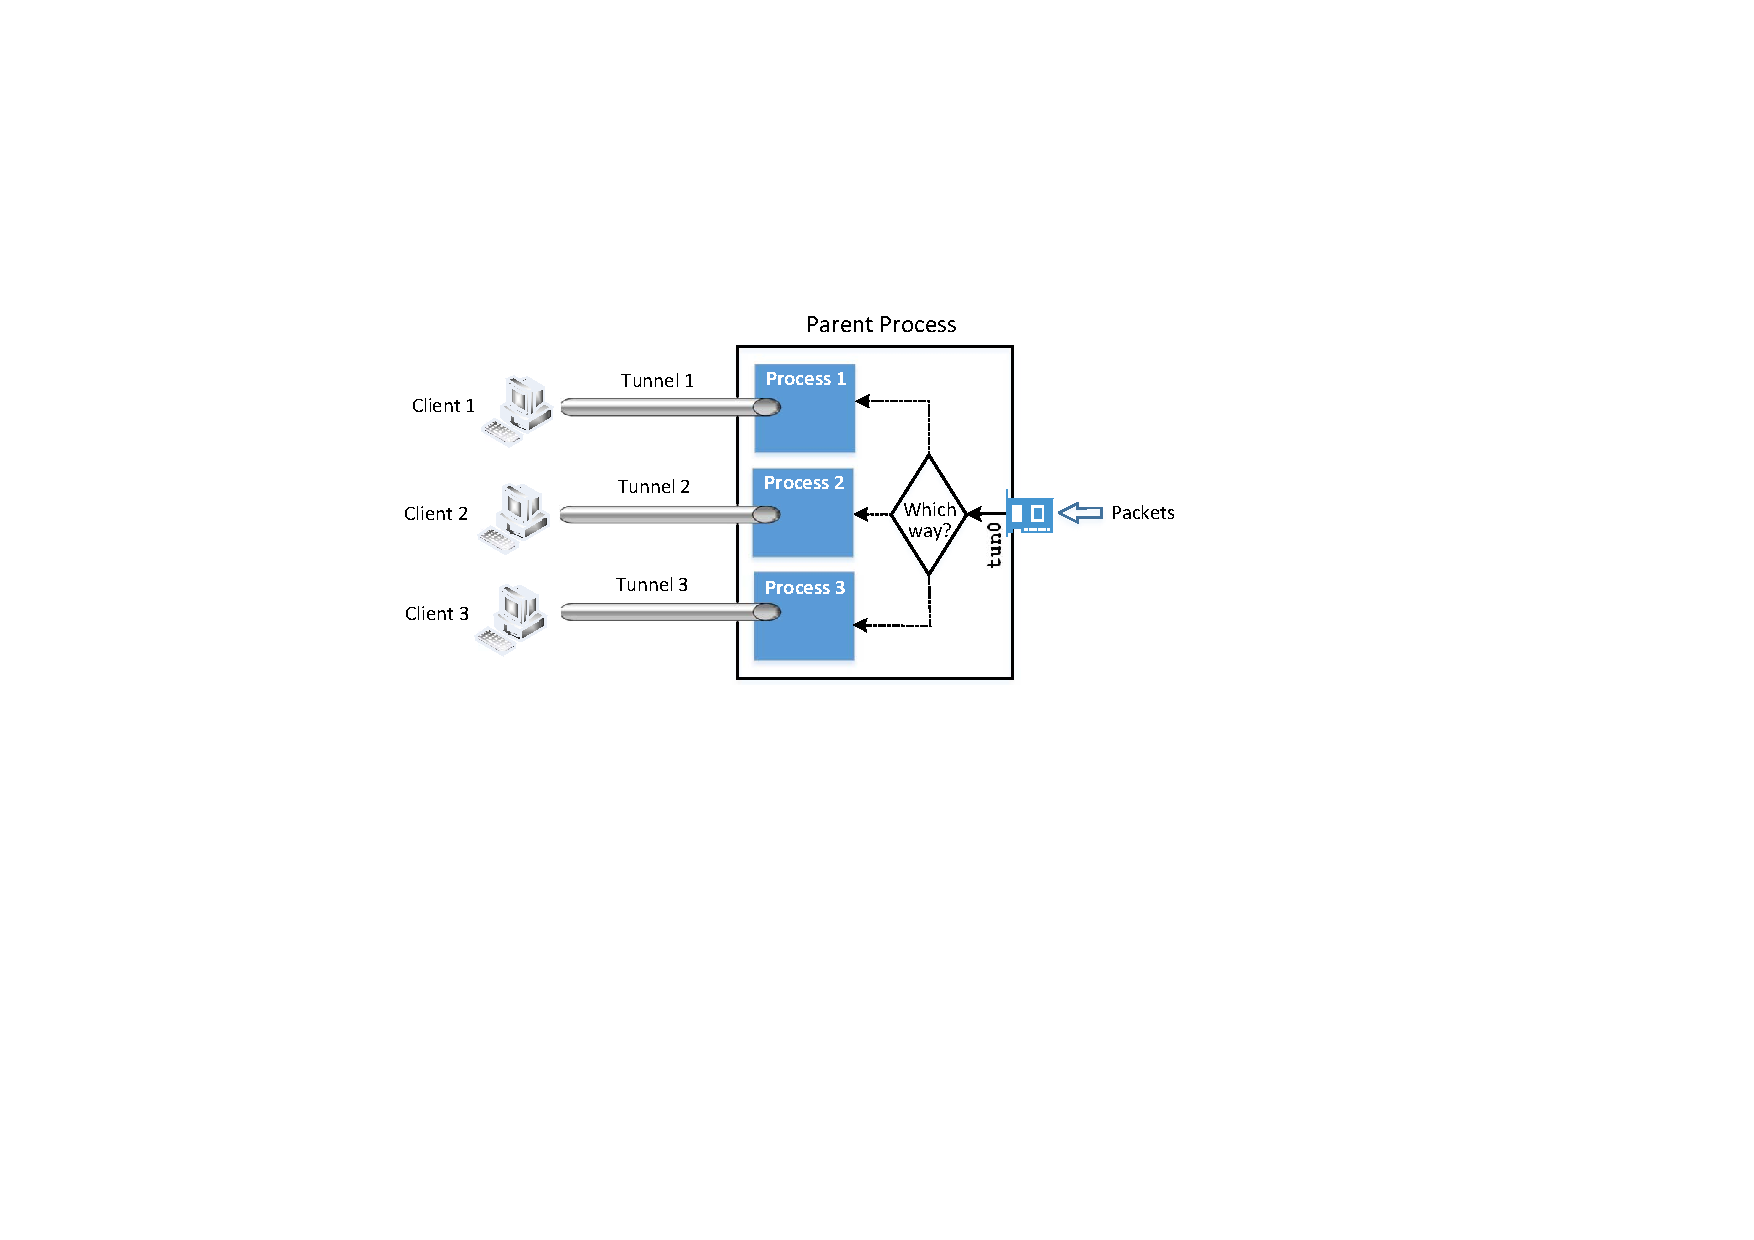
\includegraphics[width=0.8\textwidth]{\vpnFigs/MultiClient.pdf}
\end{center}
\caption{Supporting multiple VPN clients}
\label{vpn:fig:MultiClient}
\end{figure}
 

In a typical implementation, the VPN server process (the parent
process) will create a child process for each tunnel (see  
Figure~\ref{vpn:fig:MultiClient}).
When a packet comes from the tunnel, its corresponding child process 
will get the packet, and forward it to the TUN interface. 
This direction is the same regardless of whether multiple clients are 
supported or not. It is the other direction that becomes challenging. 
When a packet arrives at the TUN interface (from the private network), 
the parent process will get the packet, now it needs to figure out which
tunnel this packet should go to. You need to think about how to implement
this decision-making logic. 

Once the decision is made and a tunnel is selected, the parent process
needs to send the packet to the child process, to which
the selected tunnel is attached. This calls for IPC (Inter-Process Communication). A
typical approach is to use pipes. We provide a sample program in
Section~\ref{vpn:subsec:pipe} to demonstrate how to use pipes for IPC.


Child processes need to monitor this pipe interface, and read data from it if there 
are data. Since child processes also need to watch out for data coming from the socket
interface, they need to simultaneously monitor multiple interfaces.    
Section~\ref{vpn:subsec:select} shows how to achieve that. 




% *******************************************
% SECTION
% ******************************************* 
\section{Guidelines}



% -------------------------------------------
% SUBSECTION
% ------------------------------------------- 
\subsection{Displaying TLS Traffic in Wireshark}

Wireshark identifies TLS/SSL traffic based on port numbers. It knows 
\texttt{443} is the default port number for HTTPS, but our VPN server listens to a different
and non-standard
port number. We need to let Wireshark know that; otherwise, Wireshark will not label our 
traffic as SSL/TLS traffic. Here is what we can do: 
go to the \texttt{Edit} menu in Wireshark, and 
click  \texttt{Preferences}, \texttt{Protocols}, \texttt{HTTP}, and 
then find the \texttt{"SSL/TLS Ports"} entry. Add your SSL
server port. For example, we can change the content 
of the entry to  \texttt{443,4433}, where \texttt{4433} is the port used by our SSL server. 


\paragraph{Displaying decrypted traffic.} The approach shown above only 
gets Wireshark to recognize the traffic as TLS/SSL traffic; Wireshark cannot 
decrypt the encrypted traffic. For debugging purposes, we would like to see the decrypted
traffic. Wireshark provides such a feature; all we need to do is to provide the 
server's private key to Wireshark, and Wireshark will automatically 
derive the session keys from the TLS/SSL handshake protocol, and use these
keys to decrypt traffic. To provide the server's private key
to Wireshark, do the following:


\begin{lstlisting}
 Click Edit -> Preferences -> Protocols -> SSL 
 Find the "RSA key list", and click the Edit button
 Provide the required information about the server, see this example:
      IP Address: 10.0.2.65
      Port:       4433
      Protocol:   ssl
      Key File:   /home/seed/vpn/server-key.pem  (privat key file)
      Password:   deesdees
\end{lstlisting}


% -------------------------------------------
% SUBSECTION
% ------------------------------------------- 
\subsection{Getting IP Address from Hostname}
\label{vpn:subsec:hostnametoip}


Given a hostname, we can get the IP address for this name. 
In our sample \texttt{tlsclient} program, we use
the \texttt{gethostbyname()} function to get the IP address. However, this
function is obsolete because it does not support IPV6. 
Applications should use \texttt{getaddrinfo()} instead. The following 
example shows to how to use this function to get IP addresses. 


\begin{lstlisting}
#include <stdio.h>
#include <stdlib.h>
#include <netdb.h>
#include <netinet/in.h>
#include <sys/socket.h>
#include <arpa/inet.h>

struct addrinfo  hints, *result;

int main() {

  hints.ai_family = AF_INET; // AF_INET means IPv4 only addresses

  int error = getaddrinfo("www.example.com", NULL, &hints, &result);
  if (error) {
      fprintf(stderr, "getaddrinfo: %s\n", gai_strerror(error));
      exit(1);
  }

  // The result may contain a list of IP address; we take the first one.
  struct  sockaddr_in*  ip = (struct sockaddr_in *) result->ai_addr;
  printf("IP Address: %s\n", (char *)inet_ntoa(ip->sin_addr));

  freeaddrinfo(result);
  return 0;
}
\end{lstlisting}
 


% -------------------------------------------
% SUBSECTION
% ------------------------------------------- 
\subsection{Authentication Using the Shadow File}
\label{vpn:subsec:auth}


The following program shows how to authenticate a user using 
the account information stored in the shadow file.
The program uses \texttt{getspnam()} to get 
a given user's account information from the shadow file, including the 
hashed password. It then uses \texttt{crypt()} to 
hash a given password and see whether the result matches with
the values fetched from the shadow file. If so, the user name and the password match, 
and the authentication is successful. 


\begin{lstlisting}
#include <stdio.h>
#include <string.h>
#include <shadow.h>
#include <crypt.h>

int login(char *user, char *passwd)
{
    struct spwd *pw;
    char *epasswd;

    pw = getspnam(user);
    if (pw == NULL) {
        return -1;
    }

    printf("Login name: %s\n", pw->sp_namp);
    printf("Passwd    : %s\n", pw->sp_pwdp);

    epasswd = crypt(passwd, pw->sp_pwdp);
    if (strcmp(epasswd, pw->sp_pwdp)) {
        return -1;
    }

    return 1;
}

void main(int argc, char** argv)
{
   if (argc < 3) {
       printf("Please provide a user name and a password\n");
       return;
   }

   int r = login(argv[1], argv[2]);
   printf("Result: %d\n", r);
}
\end{lstlisting}


We can compile the code above and run it with a user name and a password. 
It should be noted that the root privilege is needed when reading from the 
shadow file. See the following commands for compilation and execution.

\begin{lstlisting}
$ gcc login.c -lcrypt
$ sudo ./a.out seed dees
\end{lstlisting}
 
It should be noted that we use \texttt{-lcrypt} in the above compilation;
we used \texttt{-lcrypto} when compiling our TLS programs. The
\texttt{crypt} and \texttt{crypto} are two different libraries, so this is
not a typo.


\vspace{0.2in}
% -------------------------------------------
% SUBSECTION
% ------------------------------------------- 
\subsection{Inter-Process Communication Using Pipe}
\label{vpn:subsec:pipe}

The following program shows how a parent process sends data to its child process using 
pipe. The parent process creates a pipe using \texttt{pipe()} in Line~\ding{192}. 
Each pipe has two ends: the input end's file descriptor is \texttt{fd[0]}, and 
the output end's file descriptor is \texttt{fd[1]}. 

After the pipe is created, a child process is spawned using \texttt{fork()}. 
Both parent and child processes have the
file descriptors associated with the pipe. They can send data to each other using the 
the pipe, which is bi-directional. However, we will only use this pipe to send data from the
parent process to the child process, and the parent will not read anything from the pipe, so 
we close the input end \texttt{fd[0]} in the parent process. Similarly, the child does not
send anything via the pipe, so it closes the output end \texttt{fd[1]}.  
At this point, we have established a uni-directional pipe from the parent process to the child process. 
To send data via the pipe, the parent process writes to \texttt{fd[1]} (see Line~\ding{193});
to receive data from the pipe, the child process reads from \texttt{fd[0]} (see
Line~\ding{194}).  



\begin{lstlisting}
#include <stdio.h>
#include <stdlib.h>
#include <unistd.h>
#include <string.h>

int main(void)
{
  int     fd[2], nbytes;
  pid_t   pid;
  char    string[] = "Hello, world!\n";
  char    readbuffer[80];

  pipe(fd);                                                  (*@\ding{192}@*)
        
  if((pid = fork()) == -1) {
       perror("fork");
       exit(1);
  }

  if(pid>0) { //parent process 
       close(fd[0]); // Close the input end of the pipe. 

       // Write data to the pipe.
       write(fd[1], string, (strlen(string)+1));             (*@\ding{193}@*)
       exit(0);
  }
  else { //child process
       close(fd[1]); // Close the output end of the pipe.

       // Read data from the pipe.
       nbytes = read(fd[0], readbuffer, sizeof(readbuffer)); (*@\ding{194}@*)
       printf("Child process received string: %s", readbuffer);
  }
  return(0);
}
\end{lstlisting}
 



% -------------------------------------------
% SUBSECTION
% ------------------------------------------- 
\subsection{Using \texttt{select} to Monitor Multiple Input Interfaces}
\label{vpn:subsec:select}

Our VPN program needs to monitor multiple interfaces, including the TUN interface, the socket
interface, and sometimes, the pipe interface.   
All these interfaces are represented by file descriptors, so we need to 
monitor them to see whether there are data coming from them. 
One way to do that is to keep polling them, and
see whether there are data on each of the interfaces. The performance of this approach is
undesirable, because the process has to keep running in an idle loop when there is no data.
Another way is to read from an interface.  By default, read is blocking, i.e., the process will
be suspended if there are no data. When data become available, the process will be unblocked,
and its execution will continue. This way, it does not waste CPU time when there is no data.

The read-based blocking mechanism works well for one interface. If a process is waiting on
multiple interfaces, it cannot block on just one of the interfaces. It has to block on all of
them altogether.  \linux has a system call called \texttt{select()}, which
allows a program to monitor multiple file descriptors simultaneously.
To use \texttt{select()}, we need to store all the file descriptors to be monitored in a set
using the \texttt{FD\_SET} macro~(see Lines~\ding{192} and~\ding{193} in
the code below).  We then give the set to the \texttt{select()} system
call~(Line~\ding{194}), which will block the process until data are available on one of the
file descriptors in the set.  We can then use the \texttt{FD\_ISSET} macro to figure out which
file descriptor has received data. In the following code example, 
we use \texttt{select()} to monitor a \texttt{TUN} and a socket file
descriptor.


\begin{lstlisting}
fd_set readFDSet;
int ret, sockfd, tunfd;

FD_ZERO(&readFDSet);
FD_SET(sockfd, &readFDSet);                                (*@\ding{192}@*)
FD_SET(tunfd, &readFDSet);                                 (*@\ding{193}@*)
ret = select(FD_SETSIZE, &readFDSet, NULL, NULL, NULL);    (*@\ding{194}@*)

if (FD_ISSET(sockfd, &readFDSet){
        // Read data from sockfd, and do something.
}

if (FD_ISSET(tunfd, &readFDSet){
        // Read data from tunfd, and do something. 
}
\end{lstlisting}



% -------------------------------------------
% SUBSECTION
% ------------------------------------------- 
\subsection{An example: using {\tt telnet} in our VPN} 

To help you fully understand how packets from an application flow to its destination
through our \miniVPN, we have drawn two figures to illustrate the complete 
packet flow path when users run {\tt telnet 10.0.20.100} from a host machine,
which is the Point A of a host-to-gateway VPN. The other end of the VPN is 
on a gateway, which is connected to the {\tt 10.0.20.0/24} network, where 
our {\tt telnet} server {\tt 10.0.20.100} resides. 


Figure~\ref{fig:example1_host_2_gateway} shows how a packet flow 
from the {\tt telnet} client to the server. 
Figure~\ref{fig:example2_host_2_gateway} shows how a packet flow 
from the {\tt telnet} server back to the client. 
We will only describe the path in Figure~\ref{fig:example1_host_2_gateway}
in the following. The return path is self-explained from
Figure~\ref{fig:example2_host_2_gateway} once you have understood 
the path in Figure~\ref{fig:example1_host_2_gateway}. 
\begin{enumerate}
\item The data of the packet starts from the {\tt telnet} program. 
\item The kernel will construct an IP packet, with the destination
      IP address being {\tt 10.0.20.100}. 
\item The kernel needs to decide which network interface the packet should 
      be routed through: {\tt eth1} or {\tt tun0}. You need to set up your routing
      table correctly for the kernel to pick {\tt tun0}. Once the decision is 
      made, the kernel will set the source IP address of the packet using
      the IP address of the network interface, which is {\tt 10.0.4.1}.

\item The packet will reach our VPN program (Point A) through the virtual 
      interface {\tt tun0}, then it will be encrypted, and then be sent back
      to the kernel through a UDP port (not through the {\tt tun0} interface).
      This is because our VPN program use the UDP as our tunnel.
      
\item The kernel will treat the encrypted IP packet as UDP data, construct
      a new IP packet, and put the entire encrypted IP packet as its UDP
      payload. The new IP's destination address will be the other end of the
      tunnel (decided by the VPN program we write); in the figure, the 
      new IP's destination address is {\tt 128.230.208.97}.


\item You need to set up your routing table correctly, so the new packet 
      will be routed through the interface {\tt eth1}; therefore, the 
      source IP address of this new packet should be {\tt 209.164.131.32}.


\item The packet will now flow through the Internet, with the original 
      {\tt telnet} packet being entirely encrypted, and carried in the 
      payload of the packet. This is why it is called a {\em tunnel}.

\item The packet will reach our gateway {\tt 128.230.208.97} through
      its interface {\tt eth1}.


\item The kernel will give the UDP payload (i.e. the encrypted IP packet)
      to the VPN program (Point B), which is waiting for UDP data. 
      This is through the UDP port.


\item The VPN program will decrypt the payload, and then feed the decrypted
      payload, which is the original {\tt telnet} packet,
      back to the kernel through the virtual network interface {\tt tun0}.

\item Since it comes through a network interface, the kernel will treat
      it as an IP packet (it is indeed an IP packet), look at its destination
      IP address, and decide where to route it. Remember, the destination
      IP address of this packet is {\tt 10.0.20.100}.
      If your routing table is 
      set up correctly, the packet should be routed through {\tt eth2},
      because this is the interface that connects to the {\tt 10.0.20.0/24}
      network. 

\item The {\tt telnet} packet will now be delivered to its final 
      destination {\tt 10.0.20.100}.




\end{enumerate}

\begin{figure*}
\centering
\begin{tabular}[t]{c}
\subfigure[An Example of packet flow from telnet client to server in Host-to-Gateway Tunnel]
{
   \label{fig:example1_host_2_gateway}
   \includegraphics*[viewport=0.7in 1.7in 8.7in 7.3in,width=6.0in]{\vpnFigs/vpn_h2g_details.pdf}
}
\\
\subfigure[An Example of packet flow from telnet server to client in Host-to-Gateway Tunnel]
{
    \label{fig:example2_host_2_gateway}
    \includegraphics*[viewport=1.6in 1.6in 9.6in 7.2in,width=6.0in]{\vpnFigs/vpn_h2g_details_reply.pdf}
}
\end{tabular}
\caption{An Example of Packet Flow in VPN.}
\label{fig:example_packetflow}
\end{figure*}





% *******************************************
% SECTION
% ******************************************* 
\section{Submission and Demonstration}


%\section*{Submission and Demonstration}


You should submit a detailed lab report to describe your design and implementation.
You should also describe how you test the functionalities and
security of your system. You also need to demonstrate your system to us. 
Please sign up a demonstration time slot with the TA. Please take
the following into consideration when you prepare for demonstraiton:

\begin{itemize}

\item The total time of the demo will be 15 minutes, no more additional time would be
given. So prepare your demonstration so you can cover the important features.  

\item You are entirely responsible for showing the demo. 
We will NOT even touch the keyboard during the
demonstration; so you should not depend on us to test your system. If you fail to demo
some important features of your system, we will assume that your system does not
have those features. 

\item You need to practice before you come to the demonstration. 
If the system crashes or anything goes wrong, it is your own fault. We will not 
debug your problems, nor give you extra time for it. 

\item 
During the demo, you should consider yourself as salesmen, and you want to sell
your system to us. You are given 15 minutes to show us how good your system is.
So think about your sales strategies. If you have implemented a great system,
but fail to show us how good it is, you are not likely to get a good grade. 

\item 
Do turn off the messages your system prints out for debugging purposes. 
Those messages should not appear in a demonstration.


\end{itemize}






% *******************************************
% SECTION
% ******************************************* 
\section{Checklist for Demonstration}


During the COVID-19 outbreak, we cannot do in-person demo. Although doing demo
online is an option, we decide to experiment with a different approach: asking students to 
record their demo and submit the video file. To help them conduct a self-guided demo,
we provide a checklist in Table~\ref{vpn:table:checklist}. Even if we do in-person demo, this checklist 
is still quite useful. 


\renewcommand{\arraystretch}{1.5}

\begin{longtable}{|p{0.2\textwidth}|p{0.8\textwidth}|}
 \caption{Checklist for VPN demonstration}
 \label{vpn:table:checklist}
 \endfirsthead
 \endhead
 \hline\xrowht[()]{10pt}
 \textbf{\Large Requirements} & \textbf{\Large Details} \\ 
 \hline
 \hline
 \textbf{Initial State} & 
	\vspace*{-0.3cm}
 	\begin{itemize}[topsep=-0.5cm,leftmargin=0.4cm]
		\item Rebooting all three VMs. Start recording after the VMs are rebooted. You
		should start demo immediately after rebooting. If you wait too long,
		you will have to do the rebooting again.

		\item Type \texttt{"last reboot; date"} in a terminal to show the rebooting
		time and current time on all three VMs. The difference between these two times
		should not be more than 5 minute.

		\item Display the routing tables on all three VMs.
	\end{itemize}
 \\ 
 \hline
 
 \textbf{Pre-Tunnel Test} & 
 	\vspace*{-0.3cm}
 	\begin{itemize}[topsep=-0.5cm,leftmargin=0.4cm]
		\item Before VPN is set up, \texttt{ping} Host \hostv
		from Host \hostu and explain your observation.
	\end{itemize}
 \\ 
 \hline

 \textbf{Tunnel Creation} & 
 	\vspace*{-0.3cm}
 	\begin{itemize}[topsep=-0.5cm,leftmargin=0.4cm]
	   \item Start vpn client and vpn server programs.
		\begin{itemize}
		\item You need to type passwords to authenticate yourself to the server, the
		password should not be visible (10 points will be deducted if we see your
		passwords). You can use \texttt{getpass()} to achieve that (type ``\texttt{man
		getpass}" to see its manual).

		\item Passwords cannot be hardcoded in your program. If you do this, 50 points will be deducted. 
		\end{itemize}

	   \item Perform configuration on all VMs. Although you can put the configuration
	   commands in a script, you do need to show the script and explain the commands in
	   your script.

	   \item Show routing tables on all three VMs after the configuration.
	\end{itemize}
 \\ 
 \hline

 \textbf{Ping Test} & 
 	\vspace*{-0.3cm}
 	\begin{itemize}[topsep=-0.5cm,leftmargin=0.4cm]
		\item On Host \hostu: \texttt{ping} Host \hostv.
		\item Use Wireshark to prove that your VPN works correctly.
		\item Show us the proof that the tunnel is indeed encrypted.
	\end{itemize}
 \\ 
 \hline

 \textbf{Telnet Test} & 
 	\vspace*{-0.3cm}
 	\begin{itemize}[topsep=-0.5cm,leftmargin=0.4cm]
		\item On Host \hostu: \texttt{telnet} to Host \hostv.
		\item Use Wireshark to prove that your VPN works correctly.
	\end{itemize}
 \\ 
 \hline

 \textbf{Tunnel-Breaking Test} & 
 	\vspace*{-0.3cm}
 	\begin{itemize}[topsep=-0.5cm,leftmargin=0.4cm]
		\item On Host \hostu, telnet to Host \hostv. While keeping the telnet connection alive,
		break the VPN tunnel by stopping the vpn client and/or vpn server programs.
		Then type something in the telnet window. Do you see what you type? What
		happens to the TCP connection? Is the connection broken? 

		\item Let us now reconnect the VPN tunnel (do not wait for too long). 
		Run the client and server programs again, and conduct the necessary
		configuration (no need to explain or show commands). Once the tunnel is
		re-established, what is going to happen to the telnet connection? Please
		describe and explain your observation.

	\end{itemize}
 \\ 
 \hline

 \textbf{Large Packet Test} & 
 	\vspace*{-0.3cm}
 	\begin{itemize}[topsep=-0.5cm,leftmargin=0.4cm]
	\item Send a large packet (size \textgreater\space 3000) from Host \hostu to Host \hostv. 
	You can use \texttt{"ping -s"} to do that. 

	\item Use Wireshark to describe and explain your observations.
	\end{itemize}
 \\ 
 \hline

 \textbf{TLS Setup} & 
 	\vspace*{-0.3cm}
 	\begin{itemize}[topsep=-0.5cm,leftmargin=0.4cm]
		\item Show us how you set up your TLS on both client and server sides.
		\item Show us where you place the server certificates and self-signed certificate.
		\item Show us which lines of code load those certificates.
	\end{itemize}
 \\ 
 \hline

 \textbf{MITM Test} & 
 	\vspace*{-0.3cm}
 	\begin{itemize}[topsep=-0.5cm,leftmargin=0.4cm]
		\item Demonstrate that your system can successfully defeat MITM attacks. You
		need to set up a simulated MITM attack, and demonstrate that your client
		program can defeat it.
	\end{itemize}
 \\ 
 \hline

 \textbf{Code Explanation 1} & 
	Which lines of code are responsible for the following:
 	\vspace*{0.2cm}
 	\begin{itemize}[topsep=-0.5cm,leftmargin=0.4cm]
		\item verifying that the server certificate is valid
		\item verifying that the server is the owner of the certificate
		\item verifying that the server is the intended server
	\end{itemize}
 \\ 
 \hline

 \textbf{Code Explanation 2} & 
	Which line of code in the client forces TLS handshake to stop if the server certificate
	verification fails?
 \\ 
 \hline

 \textbf{Code Explanation 3} & 
	Which line(s) of code do the following?
	\vspace*{0.2cm}
 	\begin{itemize}[topsep=-0.5cm,leftmargin=0.4cm]
		\item sending username and password to the server
		\item getting account information from the shadow file
	\end{itemize}
 \\ 
 \hline

 \textbf{Ending Time} & 
	Type \texttt{"last reboot; date"} commands to display the time before ending your demo.
 \\ 
 \hline

\end{longtable}



\end{document}


